\documentclass[a4j,11pt]{jarticle}
\usepackage[dvipdfmx]{graphicx}
\usepackage[report]{fireport}
\usepackage{url}

\lecture{プログラミング方法論}
\title{グリッドワールドにおけるエージェントの強化学習}
\id{情XX-XXXX}
\author{tomo-9925}
\teacher{XXXX}
%
\superhead{担当教員} %この行がなかったら,「指導教員」になります.
%
\begin{document}
\maketitle

\section{プログラムについて}

このプラグラムはじゃんけんプログラム同様Rubyで作成した.ファイルは4つに分割している.ファイルはAgentクラスをまとめた"agent.rb",Gridクラスをまとめた"grid.rb",mainを見やすくするために作った関数をまとめた"function.rb",そして定数などや全体の大まかな流れをまとめている"main.rb"で構成している.

Agentオブジェクトは指定されたグリッドオブジェクトから得られる矢印の情報をもとに進む方向を選ぶだけであり,現在の座標などのグリッドに関する情報を待たないようにしている.Gridオブジェクトはワールドに関する情報の保持とその情報の処理だけでなくエージェントの移動履歴なども管理するようにした.
Gridオブジェクトの機能としてエージェントの移動履歴を記録,その記録し情報をもとに現在地の矢印の情報の公開,矢印の大きさの更新,移動履歴の初期化,エージェントがゴールしたかの確認などの機能を有している.グリッドワールドは2次配列で表しGridオブジェクトのメンバ変数で記録している.グリッドワールドの2次元配列は配列を格納している配列をインデックスの数字の小さな方からy座標1と順に指定しており,配列内の配列は,インデックスの数字が小さな方からx座標1と順に指定している.その配列内にARROWS構造体を格納し,矢印の大きさを管理するようにした.ARROWS構造体は変数up,down,left,rightを持っており,ここにそれぞれ上下左右の矢印の大きさを格納するようにしている.今回はグリッドワールドの端のセルは座標外に移動しないように外向きを指している矢印の大きさを0とした.また,エージェントの移動履歴はLOCATION構造体を使用して管理するようにした.LOCATION構造体は変数x,y,directionを持っており,現在地のx座標とy座標と進む方向の数値を格納できるようにしている.

他に,追加機能として再現性を高めるために疑似乱数のシード値を固定させる機能,ゴールの位置をランダムにする機能,1回の実験の結果を詳しく調べるための機能,統計を取るために実験全体の実行回数を設定できる機能,エージェントの平均行動回数と平均学習時間を記録できる機能を追加した.

\newpage

\section{ソースコード}

見やすくするためにソースコードをメインの処理を書いた"main.rb"とGridクラスの定義を書いた"grid.rb",Agentクラスの定義を書いた"agent.rb",main.rbを見やすくするために分けた関数をまとめた"function.rb"の4つに分けて作成した.

\subsection{grid.rb}

\begin{verbatim}
# グリッド作成,変更,エージェントの行動の記録を行う
class Grid
  def initialize(goal)
    # @world[N][N]にArrowを格納
    @world = Array.new(N).map{Array.new(N)}
    N.times do |i|
      N.times do |j|
        if i==0 and j==0  # 左上
          @world[i][j] = ARROWS.new(0, 1.0/2, 0, 1.0/2)
        elsif i==0 and j==N-1  # 右上
          @world[i][j] = ARROWS.new(0, 1.0/2, 1.0/2, 0)
        elsif i==N-1 and j==0  # 左下
          @world[i][j] = ARROWS.new(1.0/2, 0, 0, 1.0/2)
        elsif i==N-1 and j==N-1  # 右下
          @world[i][j] = ARROWS.new(1.0/2, 0, 1.0/2, 0)
        elsif i==0  # 上
          @world[i][j] = ARROWS.new(0, 1.0/3, 1.0/3, 1.0/3)
        elsif i==N-1  # 下
          @world[i][j] = ARROWS.new(1.0/3, 0, 1.0/3, 1.0/3)
        elsif j==0  # 左
          @world[i][j] = ARROWS.new(1.0/3, 1.0/3, 0, 1.0/3)
        elsif j==N-1  # 右
          @world[i][j] = ARROWS.new(1.0/3, 1.0/3, 1.0/3, 0)
        else  # その他
          @world[i][j] = ARROWS.new(1.0/4, 1.0/4, 1.0/4, 1.0/4)
        end
      end
    end
    @start = LOCATION.new()  # LOCATION構造体で初期化
    @goal = goal
    @history = []  # 行動をエージェントの行動を記録する
  end

  # historyの初期化とスタート位置のセット
  def clear(start)
    @history.clear  # 配列を空にする
    @history << start
  end

  # historyをもとに現在地の矢印の情報を返す
  def show_arrows
    @world[@history.last[:y]][@history.last[:x]]
  end

  # Agentの場所を記録
  def record_location(direction)
    location = @history.last.dup  # 最後の位置の情報を複製
    if direction == 0
      location[:y] -= 1
    elsif direction == 1
      location[:y] += 1
    elsif direction == 2
      location[:x] -= 1
    elsif direction == 3
      location[:x] += 1
    end
    @history.last[:direction] = direction  # 移動する方向を記録
    @history << location
  end

  # 矢印の大きさを更新する
  # 考察のために使用するコードをコメントアウトしています.
  def update
    T.times do |t|
      i = @history.length - 2 - t  # 読み込むhistoryの番号
      break if i < 0  # 遡れなかったとき
    # num = T>@history.length-1 ? @history.length-1 : T  # T回遡れないとき,履歴の長さに合わせる.
    # num.times do |t|
      i = @history.length - 2 - t  # 読み込むhistoryの番号
      l = @history[i]  # 見やすくするためにポインタをコピー

      tmp1 = 1.0  - @world[l[:y]][l[:x]][l[:direction]]

      # 大きくする矢印の大きさを変更
      # @world[l[:y]][l[:x]][l[:direction]] += ( P * (num-t+1) / num )
      @world[l[:y]][l[:x]][l[:direction]] += ( P * (T-t+1) / T )
      # 1を超えたときは1にする
      @world[l[:y]][l[:x]][l[:direction]] = 1.0 if @world[l[:y]][l[:x]][l[:direction]] > 1.0

      tmp2 = 1.0  - @world[l[:y]][l[:x]][l[:direction]]

      # 小さくする矢印の大きさを変更
      4.times do |j|
        @world[l[:y]][l[:x]][j] = tmp2 * (@world[l[:y]][l[:x]][j] / tmp1) if j != l[:direction]  # tmp2==0 -> NaN
        @world[l[:y]][l[:x]][j] = 0.0 if @world[l[:y]][l[:x]][j].nan?  # NaNになったときの処理
      end
    end
  end

  # 罰を与える
  def penalty
    num = @history.length - 1
    num.times do |t|
      i = @history.length - 2 - t  # 読み込むhistoryの番号
      l = @history[i]  # 見やすくするためにポインタをコピー

      tmp1 = 1.0  - @world[l[:y]][l[:x]][l[:direction]]

      # 小さくする矢印の大きさを変更
      @world[l[:y]][l[:x]][l[:direction]] -= ( P * (num-t+1) / num )

      tmp2 = 1.0  - @world[l[:y]][l[:x]][l[:direction]]

      # 大きくする矢印の大きさを変更
      4.times do |j|
        @world[l[:y]][l[:x]][j] = tmp2 * (@world[l[:y]][l[:x]][j] / tmp1) if j != l[:direction]
      end
    end
  end

  def move_count
    @history.length-1
  end

  # 履歴を表示
  def show_history
    @history.length.times do |i|
      print "(#{(@history[i][:x]+1).to_s},#{(@history[i][:y]+1).to_s})->"
    end
    print "\b\b\n"
  end

  # グリッドの矢印の数字を整数で表示
  def show_grid
    N.times do |i|
      print "["
      N.times do |j|
        print "["
        4.times do |k|
          print "#{(@world[i][j][k]*10).floor.to_s}, "  # 切り捨てして表示
        end
        print "\b\b], "
      end
      print "\b\b],\n"
    end
    puts nil

    # グリッドの矢印を感じで表示
    N.times do |i|
      N.times do |j|
        if i == @goal[:x] and j == @goal[:y]
          print "ゴ"  # ゴールを表示
        else
          arrows = @world[i][j]
          if arrows.count(arrows.max) == 1
            case arrows.each_with_index.max[1]  # 矢印の最大値(構造体なので書き方が複雑)
            when 0
              print "上"
            when 1
              print "下"
            when 2
              print "左"
            when 3
              print "右"
            end
          else
            print "謎"
          end
        end
      end
      puts nil
    end
  end

  # Agentのhistoryをもとに現在地がゴールかを調べる
  def goal?
    @history.last == @goal
  end
end
\end{verbatim}

\newpage

\subsection{agent.rb}

\begin{verbatim}
# エージェントの作成,移動を行う
class Agent
  def initialize(grid, r)
    @grid = grid
    @r = r  # 乱数オブジェクト
  end

  # エージェントの移動
  def move
    AGENT_LIFETIME.times do |i|
      arrows = @grid.show_arrows  # gridから矢印の大きさを取得
      direction = select_direction(arrows)  # 矢印の情報をもとに移動する方向を決定
      @grid.record_location(direction)  # 決定した矢印からgridで位置を記録
      break if @grid.goal?  # ゴールしたとき処理を終了
    end
  end

  # エージェントの移動(評価用)
  def move_m
    AGENT_LIFETIME.times do |i|
      arrows = @grid.show_arrows
      direction = select_max_direction(arrows)
      @grid.record_location(direction)
      break if @grid.goal?
    end
  end

  private  # プライベートメソッド

  # 移動する方向を決定
  def select_direction(arrows)
    direction = 0
    tmp = @r.rand()  # 0~1の乱数を生成
    4.times do |i|
      tmp -= arrows[i]
      break if tmp <= 0
      direction += 1
    end
    direction
  end

  # 大きい矢印を選択
  def select_max_direction(arrows)
    direction = 0
    cnt = arrows.count(arrows.max)
    if cnt == 1
      direction = arrows.each_with_index.max[1]
    else
      tmp = @r.rand(0...cnt)
      arrows.each_with_index do |arrow, i|
        tmp -= 1 if arrow == arrows.max
        if tmp<0
          direction = i
          break
        end
      end
    end
    direction
  end
end
\end{verbatim}

\newpage

\subsection{function.rb}

\begin{verbatim}
# 定数の確認
def check_const
  if N < 2
    abort "グリッドの大きさを変更してください"
  elsif GOAL_X < 1 or N < GOAL_X
    abort "ゴールの位置を変更してください"
  elsif GOAL_Y < 1 or N < GOAL_Y
    abort "ゴールの位置を変更してください"
  elsif LEARNING_LIMIT < 1
    abort "LEARNING_LIMITを変更してください"
  elsif AGENT_LIFETIME < 1
    abort "AGENT_LIFETIMEを変更してください"
  elsif T < 0
    abort "Tを変更してください"
  elsif TRIAL_LIMIT < 1
    abort "実験回数を変更してください"
  elsif !(USE_SEED.is_a?(TrueClass) or USE_SEED.is_a?(FalseClass))
    abort "USE_SEEDに真偽値を入力してください"
  elsif !(RAND_GOAL.is_a?(TrueClass) or RAND_GOAL.is_a?(FalseClass))
    abort "RAND_GOALに真偽値を入力してください"
  elsif !(SHOW_DETAIL.is_a?(TrueClass) or SHOW_DETAIL.is_a?(FalseClass))
    abort "SHOW_DETAILに真偽値を入力してください"
  end
end

# 定数の値を出力する
def show_value
  puts "グリッドサイズ: #{N.to_s}, 学習回数: #{LEARNING_LIMIT.to_s}, エージェントの寿命: #{AGENT_LIFETIME.to_s},"
  puts "報酬: #{P.to_s}, 履歴: #{T.to_s}, 評価回数: #{VAL.to_s},"
  print "シード値: "
  if USE_SEED
    print "固定, "
  else
    print "ランダム, "
  end
  print "ゴール: "
  if RAND_GOAL
    puts "ランダム"
  else
    puts "固定"
  end
  puts nil
end

# スタートとゴールの座標を表示する
def show_location(start, goal)
  puts "スタート: (#{(start[0]+1).to_s}, #{(start[1]+1).to_s}), ゴール: (#{(goal[0]+1).to_s}, #{(goal[1]+1).to_s})"
end

# ゴールと同じ座標にならないようにスタートする座標を決定する
def set_start(goal, r)
  location = LOCATION.new(r.rand(N), r.rand(N), -1)
  while location == goal
    location = LOCATION.new(r.rand(N), r.rand(N), -1)
  end
  location
end
\end{verbatim}

\newpage

\subsection{main.rb}

\begin{verbatim}
#! /usr/bin/env ruby

# 定数
N = 5  # グリッドサイズ
GOAL_X = 1  # ゴールのX座標
GOAL_Y = 1  # ゴールのY座標
LEARNING_LIMIT = 100  # 学習回数
AGENT_LIFETIME = 30  # エージェントの寿命
P = 90e-3  # 報酬
T = 15  # 報酬で矢印を遡ることができる回数
VAL = 100   # 評価を行う回数
# オプション
USE_SEED = true  # 固定された疑似乱数を使用する
RAND_GOAL = false  # ゴール位置をランダムにする
SHOW_DETAIL = false  # 実験の結果など詳細を表示させる
TRIAL_LIMIT = 100  # 実験回数,ARROWSがTRUEのとき無効

# 構造体
ARROWS = Struct.new(:up, :down, :left, :right)
LOCATION = Struct.new(:x, :y, :direction)

# 乱数の生成
R = USE_SEED ? Random.new(150) : Random.new()  # 乱数オブジェクトの生成

# クラスと関数の読み込み
require './grid.rb'
require './agent.rb'
require './function.rb'

# メイン

check_const()  # 定数の確認
show_value() if SHOW_DETAIL  # 定数の表示

l_goal_rates = []  # 学習時のゴール率を記録していく配列
l_all_move_cnts = []  # 学習時の移動回数の平均を記録する配列列
r_goal_rates = []  # 評価時のゴール率を記録していく配列
r_all_move_cnts = []  # 評価時の移動回数の平均を記録する配列
threads = []  # スレッドを格納する配列
num = SHOW_DETAIL ? 1 : TRIAL_LIMIT  # 実験回数の決定
num.times do |t|
  threads << Thread.start do
    # 実験に使用する乱数オブジェクトの生成
    r = Random.new(R.rand(0...1000000))
    # ゴールの座標を決める
    goal = RAND_GOAL ? LOCATION.new(r.rand(N), r.rand(N), -1) : LOCATION.new(GOAL_X-1, GOAL_Y-1, -1)
    # directionの初期値は-1とする
    grid = Grid.new(goal)  # グリッドワールドの作成

    # 学習
    goal_cnt = 0  # ゴール回数を記録
    move_cnts = []
    LEARNING_LIMIT.times do |i|
      start = set_start(goal, r)  # スタート位置を決定
      grid.clear(start)  # グリッドのhistoryの初期化とスタート位置のセット
      agent = Agent.new(grid, r)  # エージェントの初期化
      agent.move  # エージェントを移動させる
      move_cnts << grid.move_count  # エージェントの移動回数を記録
      # grid.show_history if SHOW_DETAIL  # エージェントの履歴を表示する
      if grid.goal?  # もしエージェントがゴールしたとき
        # puts "ゴールしました" if SHOW_DETAIL
        grid.update  # グリッドの矢印を更新する
        goal_cnt += 1  # ゴール回数をカウントする
      else
        # puts "ゴールできませんでした" if SHOW_DETAIL
        # grid.penalty  # 罰を与える
      end
      # puts nil if SHOW_DETAIL  # 改行
    end
    l_all_move_cnts << move_cnts.inject(:+)/move_cnts.length.to_f  # 移動回数の平均を記録
    l_goal_rates << goal_cnt/LEARNING_LIMIT.to_f  # ゴール率を記録
    grid.show_grid if SHOW_DETAIL  # グリッドの情報を表示

    # 評価
    goal_cnt = 0
    move_cnts = []
    VAL.times do |i|
      start = set_start(goal, r)
      grid.clear(start)
      agent = Agent.new(grid, r)
      agent.move_m
      move_cnts << grid.move_count
      goal_cnt += 1 if grid.goal?
    end
    r_all_move_cnts << move_cnts.inject(:+)/move_cnts.length.to_f
    r_goal_rates << goal_cnt/VAL.to_f
  end
end

# すべてのスレッドが終了するのを待つ
threads.each do |thr|
  thr.join
end

# 結果の表示
if SHOW_DETAIL
  puts nil
  puts "学習時のゴール率: #{l_goal_rates.last.to_s}"
  puts "学習時のエージェントの平均行動回数: #{l_all_move_cnts.last.to_s}"
  puts "学習後のゴール率: #{r_goal_rates.last.to_s}"
  puts "学習後のエージェントの平均行動回数: #{r_all_move_cnts.last.to_s}"
else
  # 学習中
  p l_goal_rates.max  # 最大値
  p l_goal_rates.inject(:+)/l_goal_rates.length  # 平均値
  p l_goal_rates.min  # 最小値
  p l_all_move_cnts.inject(:+)/l_all_move_cnts.length  # 移動回数の平均
  # 学習後
  p r_goal_rates.max  # 最大値
  p r_goal_rates.inject(:+)/r_goal_rates.length  # 平均値
  p r_goal_rates.min  # 最小値
  p r_all_move_cnts.inject(:+)/l_all_move_cnts.length  # 移動回数の平均
end
\end{verbatim}

\newpage

\section{パラメータ}

私は機械学習や統計の知識がないので,エージェントの寿命をグリッドワールドの大きさによって可変的に変更するようにするべきかどうかなどがわからなかったため,ひとまず,すべての数値を固定とした.以下の数値がこれから行う考察のデフォルト値である.

\begin{verbatim}
$ cat ./main.rb | head -n 16 | tail -n 14
# 定数
N = 5  # グリッドサイズ
GOAL_X = 1  # ゴールのX座標
GOAL_Y = 1  # ゴールのY座標
LEARNING_LIMIT = 100  # 学習回数
AGENT_LIFETIME = 30  # エージェントの寿命
P = 1e-2  # 報酬
T = 15  # 報酬で矢印を遡ることができる回数
VAL = 100   # 評価でを行う回数
# オプション
USE_SEED = true  # 固定された疑似乱数を使用する
RAND_GOAL = false  # ゴール位置をランダムにする
SHOW_DETAIL = false  # 実験の結果など詳細を表示させる
TRIAL_LIMIT = 100  # 実験回数,ARROWSがTRUEのとき無効
\end{verbatim}

グリッドサイズは5で,ゴールの位置は図で言うと左上である.学習回数は500回とし,エージェントの寿命は15とした.また,報酬は$1.0×10^{-2}$で,遡ることができる回数は15とした.考察ではシード値を固定し,評価を100回行った.TRIAL\_LIMITを100に設定して100回学習を行い,そこからゴール率の最大値と最小値,平均値,エージェントの平均移動回数,学習時間の平均を計算し比較を行った.

\newpage

\section{考察}

\subsection{パラメータと学習のしやすさ}

実験結果の詳細なデータは\url{https://kutc-my.sharepoint.com/:x:/g/personal/k992077_kansai-u_ac_jp/EdlxfqMy4PVLgDlh8IxcRj4BJc7dcYQ50wBGp1RkpnDvdw?e=9LY8Pv}に公開している.

\subsubsection{グリッドワールドの広さと学習のしやすさ}

この関係を調べるために上記で記したデフォルト値からグリッドワールドの大きさを表す定数Nの数値を1から20まで順に1ずつ上げていき,ゴール率と学習1回あたりのエージェントの平均行動回数,学習時間の平均がどのように変化するか調べた.結果は以下のようになった.

\begin{figure}[ht]
  \begin{center}
    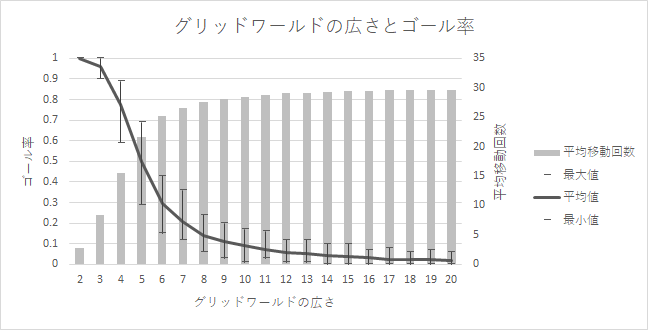
\includegraphics[scale=1.5]{img/changeN.png}
  \end{center}
\end{figure}

学習1回あたりエージェントの平均行動回数と学習時間の平均はグリッドワールドを大きくするほど増加していった.ゴール率の平均値の推移を見ていくとグリッドワールドの大きさを広くすればするほどゴール率が低くなる傾向があった.

実際の学習結果を見るためにグリッドワールドの大きさを10とし,シード値をランダムにし,学習結果の詳細を表示させてみた.結果は以下の通りとなった.

\newpage

\begin{verbatim}
グリッドサイズ: 10, 学習回数: 100, エージェントの寿命: 30,
報酬: 0.01, 報酬で遡ることができる回数: 15,
シード値: ランダム, ゴール: 固定

[[0, 5, 0, 5], [0, 3, 3, 3], [0, 3, 3, 3], [0, 3, 3, 3], [0, 3, 3, 3], [0, 3, 3, 3], [0, 3, 3, 3], [0, 3, 3, 3], [0, 3, 3, 3], [0, 5, 5, 0]],
[[3, 3, 0, 3], [2, 2, 2, 2], [2, 2, 2, 2], [2, 2, 2, 2], [2, 2, 2, 2], [2, 2, 2, 2], [2, 2, 2, 2], [2, 2, 2, 2], [2, 2, 2, 2], [3, 3, 3, 0]],
[[3, 3, 0, 3], [2, 2, 2, 2], [2, 2, 2, 2], [2, 2, 2, 2], [2, 2, 2, 2], [2, 2, 2, 2], [2, 2, 2, 2], [2, 2, 2, 2], [2, 2, 2, 2], [3, 3, 3, 0]],
[[3, 3, 0, 3], [2, 2, 2, 2], [2, 2, 2, 2], [2, 2, 2, 2], [2, 2, 2, 2], [2, 2, 2, 2], [2, 2, 2, 2], [2, 2, 2, 2], [2, 2, 2, 2], [3, 3, 3, 0]],
[[3, 3, 0, 3], [2, 2, 2, 2], [2, 2, 2, 2], [2, 2, 2, 2], [2, 2, 2, 2], [2, 2, 2, 2], [2, 2, 2, 2], [2, 2, 2, 2], [2, 2, 2, 2], [3, 3, 3, 0]],
[[3, 3, 0, 3], [2, 2, 2, 2], [2, 2, 2, 2], [2, 2, 2, 2], [2, 2, 2, 2], [2, 2, 2, 2], [2, 2, 2, 2], [2, 2, 2, 2], [2, 2, 2, 2], [3, 3, 3, 0]],
[[3, 3, 0, 3], [2, 2, 2, 2], [2, 2, 2, 2], [2, 2, 2, 2], [2, 2, 2, 2], [2, 2, 2, 2], [2, 2, 2, 2], [2, 2, 2, 2], [2, 2, 2, 2], [3, 3, 3, 0]],
[[3, 3, 0, 3], [2, 2, 2, 2], [2, 2, 2, 2], [2, 2, 2, 2], [2, 2, 2, 2], [2, 2, 2, 2], [2, 2, 2, 2], [2, 2, 2, 2], [2, 2, 2, 2], [3, 3, 3, 0]],
[[3, 3, 0, 3], [2, 2, 2, 2], [2, 2, 2, 2], [2, 2, 2, 2], [2, 2, 2, 2], [2, 2, 2, 2], [2, 2, 2, 2], [2, 2, 2, 2], [2, 2, 2, 2], [3, 3, 3, 0]],
[[5, 0, 0, 5], [3, 0, 3, 3], [3, 0, 3, 3], [3, 0, 3, 3], [3, 0, 3, 3], [3, 0, 3, 3], [3, 0, 3, 3], [3, 0, 3, 3], [3, 0, 3, 3], [5, 0, 5, 0]],

ゴ下左左左左謎謎謎謎
上上上上謎上左左謎謎
上左下上謎謎謎謎謎謎
上上左謎謎謎謎謎謎謎
上謎謎謎謎謎謎謎謎謎
謎謎謎謎謎謎謎謎謎謎
謎謎謎謎謎謎謎謎謎謎
謎謎謎謎謎謎謎謎謎謎
謎謎謎謎謎謎謎謎謎謎
謎謎謎謎謎謎謎謎謎謎

ゴール率: 0.06
エージェントの平均行動回数: 28.87
学習にかかった時間: 0.005843999999342486
\end{verbatim}

寿命が短いためゴールから距離が離れ過ぎているとゴールができないことがあることがわかる.また,学習し始めのときであれば,寿命がゴールまでもったとしても矢印の大きさがすべて等しいため,逆方向に行くこともありゴールできない可能性が高い.よって,ゴールグリッドワールドは小さいほうが学習しやすいと考えられる.

\newpage

\subsubsection{ゴールの位置と学習のしやすさ}

この関係を調べるためにデフォルト値からゴールの位置のx座標である定数GOAL\_Xの値を1から5,y座標である定数GOAL\_Yの値を1から5をそれぞれ選択し,すべての組み合わせで実験を行いゴール率と学習1回あたりエージェントの平均行動回数,学習時間の平均を比較した.結果は以下のようになった.

\begin{figure}[ht]
  \begin{center}
    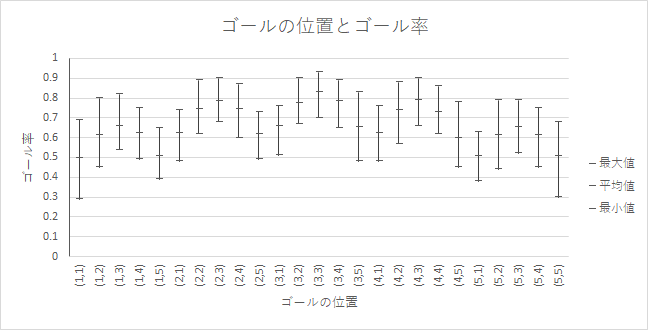
\includegraphics[scale=1.5]{img/changeGoal.png}
  \end{center}
\end{figure}

一番ゴール率の平均値が高いのは(3,3)で,それに続き平均値が高いのは(4,3),(3,4),(2,3),(3,2)であった.また,学習1回あたりエージェントの平均行動回数はグリッドワールドの中央ほど少なくなっていた.

エージェントをグリッドワールドのどこかしらの角からスタートさせ,ゴールを対角線上の角に置く場合と中心に置く場合を考えると,最短経路を辿ったとしてもエージェントの移動距離に倍の差が生まれる.グリッドワールドの大きさとゴール率の実験でわかった通り,ゴールとスタートの距離が離れれば離れるほどゴール率が低くなるため,ゴール率や学習の効率を上げるためにはゴールをグリッドワールドの中心の方に設定することが有効な方法だと考えられる.

\newpage

\subsubsection{履歴の長さと学習のしやすさ}

グラフをわかりやすくするため,この関係を調べるために定数を以下のように設定し,定数Tの数値を0から30まで順に1ずつ上げていきゴール率と学習1回あたりエージェントの平均行動回数,学習時間の平均がどのように変化するか調べた.結果は以下のようになった.

\begin{verbatim}
# 定数
N = 10  # グリッドサイズ
GOAL_X = 5  # ゴールのX座標
GOAL_Y = 5  # ゴールのY座標
LEARNING_LIMIT = 500  # 学習回数
AGENT_LIFETIME = 30  # エージントの寿命
P = 1e-2  # 報酬
\end{verbatim}

\begin{figure}[ht]
  \begin{center}
    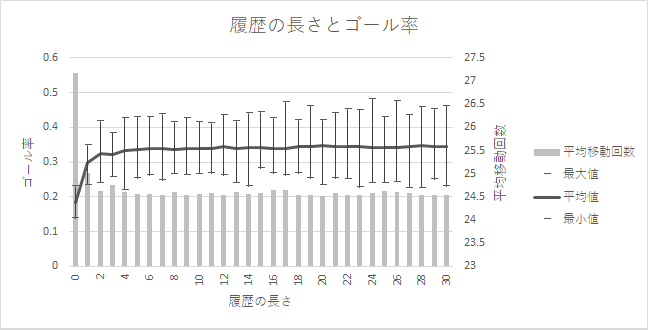
\includegraphics[scale=1.5]{img/changeT.png}
  \end{center}
\end{figure}

履歴の長さが0から6まではゴール率は増加,平均行動率は減少する傾向があり,それ以降はゴール率がほぼ変化しない結果となった.また,履歴の長さを長くするほど学習時間が伸びる傾向があった.

詳細な内容を調べるために定数を上記のものからシード値をランダムにして学習結果の詳細を表示させ,Tの値を15と100にそれぞれ変更してみた.結果は以下の通りとなった.

\newpage

\begin{verbatim}
グリッドサイズ: 10, 学習回数: 500, エージェントの寿命: 30,
報酬: 0.01, 報酬で遡ることができる回数: 5,
シード値: ランダム, ゴール: 固定

[[0, 5, 0, 5], [0, 3, 3, 3], [0, 3, 3, 3], [0, 3, 3, 3], [0, 3, 3, 3], [0, 3, 3, 3], [0, 3, 3, 3], [0, 3, 3, 3], [0, 3, 3, 3], [0, 5, 5, 0]],
[[3, 3, 0, 3], [2, 2, 2, 2], [2, 2, 2, 2], [2, 2, 2, 2], [2, 2, 2, 2], [2, 2, 2, 2], [2, 2, 2, 2], [2, 2, 2, 2], [2, 2, 2, 2], [3, 3, 3, 0]],
[[3, 3, 0, 3], [2, 2, 2, 2], [2, 2, 2, 2], [2, 2, 2, 2], [1, 3, 2, 2], [2, 2, 2, 2], [2, 2, 2, 2], [2, 2, 2, 2], [2, 2, 2, 2], [3, 3, 3, 0]],
[[3, 3, 0, 3], [2, 2, 2, 2], [2, 2, 2, 3], [1, 2, 1, 3], [0, 6, 1, 1], [1, 2, 3, 1], [2, 2, 3, 2], [2, 2, 2, 2], [2, 2, 2, 2], [3, 3, 3, 0]],
[[3, 3, 0, 3], [2, 2, 2, 2], [2, 2, 2, 3], [0, 1, 0, 6], [2, 2, 2, 2], [1, 1, 6, 1], [2, 2, 3, 2], [2, 2, 2, 2], [2, 2, 2, 2], [3, 3, 3, 0]],
[[3, 3, 0, 3], [2, 2, 2, 2], [2, 2, 2, 3], [3, 1, 1, 3], [6, 1, 1, 1], [3, 1, 3, 1], [2, 2, 2, 2], [2, 2, 2, 2], [2, 2, 2, 2], [3, 3, 3, 0]],
[[3, 3, 0, 3], [2, 2, 2, 2], [2, 2, 2, 2], [3, 2, 2, 2], [3, 1, 2, 1], [3, 2, 2, 2], [2, 2, 2, 2], [2, 2, 2, 2], [2, 2, 2, 2], [3, 3, 3, 0]],
[[3, 3, 0, 3], [2, 2, 2, 2], [2, 2, 2, 2], [2, 2, 2, 2], [2, 2, 2, 2], [2, 2, 2, 2], [2, 2, 2, 2], [2, 2, 2, 2], [2, 2, 2, 2], [3, 3, 3, 0]],
[[3, 3, 0, 3], [2, 2, 2, 2], [2, 2, 2, 2], [2, 2, 2, 2], [2, 2, 2, 2], [2, 2, 2, 2], [2, 2, 2, 2], [2, 2, 2, 2], [2, 2, 2, 2], [3, 3, 3, 0]],
[[5, 0, 0, 5], [3, 0, 3, 3], [3, 0, 3, 3], [3, 0, 3, 3], [3, 0, 3, 3], [3, 0, 3, 3], [3, 0, 3, 3], [3, 0, 3, 3], [3, 0, 3, 3], [5, 0, 5, 0]],

謎謎謎下謎謎謎謎謎謎
謎謎右下下下謎謎謎謎
謎謎下下下下下左謎謎
謎右右右下左左下左謎
右右右右ゴ左左左左謎
上右右上上左左左左謎
謎上上上上上上謎謎謎
謎謎上上上上左謎謎謎
謎謎謎謎上上謎謎謎謎
謎謎謎謎謎謎謎謎謎謎

ゴール率: 0.302
エージェントの平均行動回数: 25.29
学習にかかった時間: 0.026163000002270564
\end{verbatim}

\newpage

\begin{verbatim}
グリッドサイズ: 10, 学習回数: 500, エージェントの寿命: 30,
報酬: 0.01, 報酬で遡ることができる回数: 20,
シード値: ランダム, ゴール: 固定

[[0, 5, 0, 4], [0, 3, 3, 3], [0, 3, 3, 3], [0, 3, 3, 3], [0, 3, 3, 3], [0, 3, 3, 3], [0, 3, 3, 3], [0, 3, 3, 3], [0, 3, 3, 3], [0, 4, 5, 0]],
[[3, 3, 0, 3], [2, 2, 2, 2], [2, 2, 2, 2], [2, 2, 2, 2], [1, 3, 2, 2], [2, 2, 3, 2], [2, 2, 2, 2], [2, 2, 2, 2], [2, 2, 2, 2], [3, 3, 3, 0]],
[[3, 3, 0, 3], [2, 2, 2, 2], [2, 2, 2, 2], [2, 2, 2, 2], [1, 3, 2, 1], [2, 2, 2, 2], [2, 2, 2, 2], [2, 2, 2, 2], [2, 2, 2, 2], [3, 3, 3, 0]],
[[3, 3, 0, 3], [2, 2, 2, 2], [2, 3, 1, 2], [1, 3, 1, 3], [0, 6, 1, 1], [1, 2, 4, 1], [2, 2, 3, 2], [2, 3, 2, 2], [2, 2, 2, 2], [3, 3, 3, 0]],
[[2, 3, 0, 3], [2, 2, 2, 3], [1, 1, 1, 5], [0, 0, 1, 7], [2, 2, 2, 2], [1, 1, 6, 1], [1, 1, 5, 1], [1, 2, 3, 2], [2, 2, 3, 2], [3, 3, 3, 0]],
[[3, 3, 0, 3], [2, 2, 2, 2], [2, 1, 2, 3], [2, 2, 2, 3], [5, 1, 1, 1], [3, 2, 2, 1], [2, 2, 2, 2], [2, 2, 3, 2], [2, 2, 2, 2], [3, 3, 3, 0]],
[[3, 3, 0, 3], [2, 2, 2, 2], [2, 2, 2, 2], [2, 2, 2, 3], [5, 1, 1, 1], [4, 2, 1, 1], [2, 1, 3, 2], [2, 2, 3, 2], [2, 2, 2, 2], [3, 3, 3, 0]],
[[3, 3, 0, 3], [2, 2, 2, 2], [2, 2, 2, 2], [3, 2, 2, 2], [2, 2, 2, 2], [4, 1, 1, 2], [2, 2, 2, 2], [2, 2, 2, 2], [2, 2, 2, 2], [3, 3, 3, 0]],
[[3, 3, 0, 3], [2, 2, 2, 2], [2, 2, 2, 2], [2, 2, 2, 2], [2, 2, 2, 2], [2, 2, 2, 2], [2, 2, 2, 2], [2, 2, 2, 2], [2, 2, 2, 2], [3, 3, 3, 0]],
[[5, 0, 0, 5], [3, 0, 3, 3], [3, 0, 3, 3], [3, 0, 3, 3], [3, 0, 3, 3], [3, 0, 3, 3], [3, 0, 3, 3], [3, 0, 3, 3], [3, 0, 3, 3], [5, 0, 4, 0]],

下下右下下下下左左左
右下下右下左左左下下
下右下下下下左下左左
下右下下下左左下下左
右右右右ゴ左左左左左
上右右右上上左左左左
右上上右上上左左左左
右上右上上上上左左左
上上上右上上左左上上
謎右上上左上左右右上

ゴール率: 0.396
エージェントの平均行動回数: 23.99
学習にかかった時間: 0.03213600002345629
\end{verbatim}

\newpage

矢印の大きさを数値で見ていると,履歴の長さを短く設定しているときは中心付近の矢印の大きさが大きくなっており遠回りがないのに対し,履歴の長さを長く設定しているときは全体的に数値が変化しておらず遠回りがあることがわかる.この結果から,履歴の長さが短いとゴールのすぐ近くを通るまで動き回り続ける可能性があり,履歴の長さが長いと全体的にゴールには行きやすくなるが回り道をする確率が高まり動き回り続ける可能性が高くなることが予想できる.このことから,履歴の長さは短すぎず長すぎない,ゴールから一番離れたセルの矢印の大きさが変わるくらいに設定するのが良いと思われる.

\newpage

\subsubsection{エージェントの寿命の適切な長さ}

この関係を調べるためにデフォルト値からエージェントの寿命を表す定数AGENT\_LIFETIMEの数値を5から200まで順に5ずつ上げていきゴール率と学習1回あたりエージェントの平均行動回数,学習時間の平均がどのに変化していくか調べた.結果は以下のようになった.

\begin{figure}[ht]
  \begin{center}
    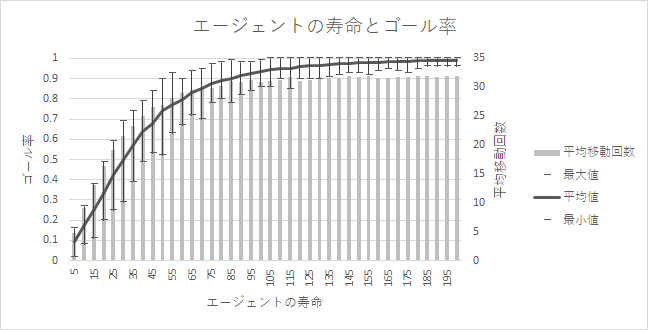
\includegraphics[scale=1.5]{img/changeAgentLifetime.png}
  \end{center}
\end{figure}

エージェントの寿命を長くさせるほどゴール率と学習1回あたりエージェントの平均行動回数,1回の実験あたりの学習時間の平均がすべて増加する傾向があった.

詳細な内容を調べるためにエージェントの寿命を10と40に設定し学習結果の詳細を表示させてみた.結果は以下の通りとなった.

\begin{verbatim}
グリッドサイズ: 5, 学習回数: 100, エージェントの寿命: 10,
報酬: 0.01, 報酬で遡ることができる回数: 15,
シード値: 固定, ゴール: 固定

[[0, 5, 0, 5], [0, 2, 4, 2], [0, 2, 4, 3], [0, 3, 3, 3], [0, 4, 5, 0]],
[[3, 3, 0, 3], [2, 2, 2, 2], [2, 2, 2, 2], [2, 2, 2, 2], [3, 3, 3, 0]],
[[3, 3, 0, 3], [2, 2, 2, 2], [2, 2, 2, 2], [2, 2, 2, 2], [3, 3, 3, 0]],
[[3, 3, 0, 3], [2, 2, 2, 2], [2, 2, 2, 2], [2, 2, 2, 2], [3, 3, 3, 0]],
[[5, 0, 0, 4], [3, 0, 3, 3], [3, 0, 3, 3], [3, 0, 3, 3], [5, 0, 5, 0]],

ゴ左左左左
上上左左左
上上右上上
上左下謎謎
上左左謎謎

ゴール率: 0.21
エージェントの平均行動回数: 8.99
学習にかかった時間: 0.005109000019729137
\end{verbatim}

\newpage

\begin{verbatim}
グリッドサイズ: 5, 学習回数: 100, エージェントの寿命: 40,
報酬: 0.01, 報酬で遡ることができる回数: 15,
シード値: 固定, ゴール: 固定

[[0, 5, 0, 5], [0, 1, 6, 1], [0, 2, 5, 2], [0, 2, 4, 2], [0, 3, 6, 0]],
[[4, 2, 0, 2], [3, 1, 3, 1], [2, 2, 3, 1], [3, 2, 2, 2], [3, 3, 3, 0]],
[[4, 2, 0, 2], [3, 2, 2, 2], [2, 2, 2, 2], [2, 2, 2, 2], [3, 3, 3, 0]],
[[3, 2, 0, 3], [2, 2, 2, 2], [2, 2, 2, 2], [2, 2, 2, 2], [3, 3, 3, 0]],
[[5, 0, 0, 4], [3, 0, 3, 2], [3, 0, 3, 3], [3, 0, 3, 3], [4, 0, 5, 0]],

ゴ左左左左
上上左上上
上上上上上
上上左右左
上上上左左

ゴール率: 0.59
エージェントの平均行動回数: 26.64
学習にかかった時間: 0.016950000019278377
\end{verbatim}

以上の結果から,ゴール率が低くエージェントの寿命がある程度短くても学習はうまく行くことがわかる.しかし,エージェントの寿命が短すぎる場合は学習されないセルが出て来ることが多く,長すぎた場合は学習時間の平均が増える上に遠回りとなるルートを学習する可能性が上がるため,実際に学習の結果を見て適度な長さを考えて設定する必要がある.

\newpage

\subsubsection{学習回数の適切な回数}

この関係を調べるためにデフォルト値から学習回数を表す定数LEARNING\_LIMITの数値を100から2000まで順に100ずつ上げていきゴール率と学習1回あたりエージェントの平均行動回数,学習時間がどのに変化していくか調べた.結果は以下のようになった.

\begin{figure}[ht]
  \begin{center}
    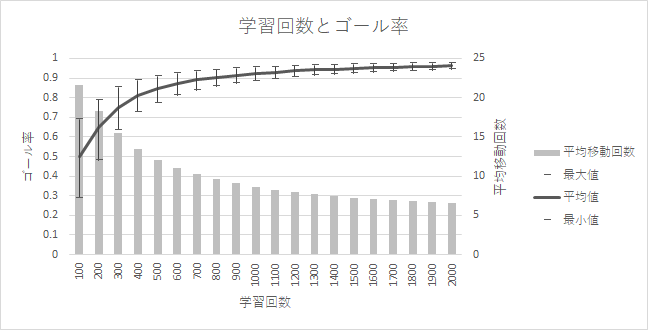
\includegraphics[scale=1.5]{img/changeLearningLimit.png}
  \end{center}
\end{figure}

学習回数を増やすほどゴール率と学習時間の平均が上がり,平均行動回数は下がる傾向があった.

詳細な内容を調べるために学習回数を200と2000に,シード値をランダムに設定し学習結果の詳細を表示させた.結果は以下のようになった.

\begin{verbatim}
グリッドサイズ: 5, 学習回数: 200, エージェントの寿命: 30,
報酬: 0.01, 報酬で遡ることができる回数: 15,
シード値: ランダム, ゴール: 固定

[[0, 5, 0, 5], [0, 0, 10, 0], [0, 0, 9, 0], [0, 2, 5, 2], [0, 4, 5, 0]],
[[6, 1, 0, 2], [4, 1, 3, 1], [4, 1, 2, 1], [2, 1, 3, 2], [3, 2, 3, 0]],
[[5, 2, 0, 2], [3, 1, 2, 2], [4, 1, 2, 1], [2, 1, 3, 2], [3, 2, 3, 0]],
[[4, 2, 0, 2], [3, 1, 3, 2], [3, 2, 2, 2], [2, 2, 2, 2], [3, 3, 3, 0]],
[[5, 0, 0, 4], [3, 0, 3, 3], [3, 0, 3, 3], [3, 0, 3, 3], [4, 0, 5, 0]],

ゴ左左左左
上上上左左
上上上左左
上上上上上
上上上左左

ゴール率: 0.685
エージェントの平均行動回数: 17.88
学習にかかった時間: 0.019226000003982335
\end{verbatim}

\newpage

\begin{verbatim}
グリッドサイズ: 5, 学習回数: 2000, エージェントの寿命: 30,
報酬: 0.01, 報酬で遡ることができる回数: 15,
シード値: ランダム, ゴール: 固定

[[0, 5, 0, 5], [0, 0, 10, 0], [0, 0, 10, 0], [0, 0, 10, 0], [0, 0, 10, 0]],
[[10, 0, 0, 0], [10, 0, 0, 0], [5, 0, 4, 0], [0, 0, 10, 0], [2, 1, 6, 0]],
[[10, 0, 0, 0], [10, 0, 0, 0], [0, 0, 10, 0], [0, 0, 10, 0], [0, 0, 10, 0]],
[[10, 0, 0, 0], [10, 0, 0, 0], [10, 0, 0, 0], [9, 0, 0, 0], [7, 0, 2, 0]],
[[10, 0, 0, 0], [4, 0, 3, 1], [10, 0, 0, 0], [2, 0, 5, 1], [4, 0, 5, 0]],

ゴ左左左左
上上上左左
上上左左左
上上上上上
上上上左左

ゴール率: 0.969
エージェントの平均行動回数: 6.4505
学習にかかった時間: 0.10161200002767146
\end{verbatim}

これらの結果を比べてみると,学習回数が2000のときは多くのセルで矢印の大きさが10になっているものが多く見られる.このことから,学習回数を増やすと矢印の大きさが大きくなり,良い学習となることがわかる.よって,学習時間を気にしないのであれば,学習回数は多い方が良いと思われる.

\newpage

\subsubsection{報酬の変更による影響} %傾向

この関係を調べるためにデフォルト値から報酬を表す定数Pの数値を$0$から$9e-2$まで順に$1e-3$ずつ上げていきゴール率とエージェントの平均行動回数,学習時間の平均がどのに変化していくか調べた.結果は以下のようになった.

\begin{figure}[ht]
  \begin{center}
    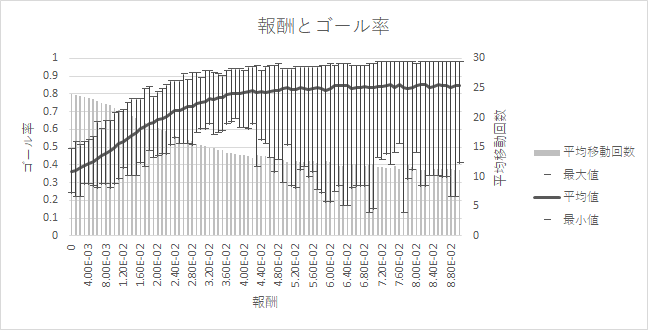
\includegraphics[scale=1.5]{img/changeP.png}
  \end{center}
\end{figure}

報酬を多く与えるほどゴール率の平均が上がり,平均移動回数は下がった.また,途中からゴール率の最低値が著しく下がり,ゴール率があまり変化しなくなる結果となった.

詳細な内容を調べるために報酬の量を$8e-2$,シード値をランダムにして学習結果の詳細を表示せる設定で数十回プログラムを実行させたところ以下のような結果が得られた.

\begin{verbatim}
  グリッドサイズ: 5, 学習回数: 100, エージェントの寿命: 30,
  報酬: 0.08, 報酬で遡ることができる回数: 15,
  シード値: ランダム, ゴール: 固定

  [[0, 5, 0, 5], [0, 0, 0, 10], [0, 0, 10, 0], [0, 4, 2, 3], [0, 5, 4, 0]],
  [[10, 0, 0, 0], [0, 2, 4, 2], [1, 0, 6, 1], [1, 1, 4, 1], [2, 3, 4, 0]],
  [[10, 0, 0, 0], [0, 3, 5, 0], [2, 1, 4, 1], [0, 6, 1, 1], [2, 2, 4, 0]],
  [[10, 0, 0, 0], [0, 0, 10, 0], [0, 0, 8, 0], [2, 1, 5, 0], [1, 2, 5, 0]],
  [[9, 0, 0, 0], [3, 0, 3, 2], [5, 0, 3, 0], [1, 0, 5, 2], [5, 0, 4, 0]],

  ゴ右左下下
  上左左左左
  上左左下左
  上左左左左
  上左上左上

  ゴール率: 0.61
  エージェントの平均行動回数: 18.07
  学習にかかった時間: 0.00911500002257526
\end{verbatim}

\newpage

結果を見てみると,右側の方の学習がうまくできておらず,セルの一部では誤った学習がされていることがわかる.一度良くないルートを学習して,その後そのルートに支配されるようになり,このような結果になったと考えられる.この結果から,報酬は少なすぎると矢印の大きさがほぼ変化せず矢印の方向を決定しづらくるため,報酬は他のパラメータに合わせて上記の現象が起こらない適度に設定する必要がある.

\newpage

\subsection{矢印の長さの更新ルールをどのように変更すると効果的か}

% 式(1)の矢印の長さの更新ルールをどのように変更すると効果的か?
% 式(1)では,ステップ数を遡るほど報酬が少なく分配されている.
% 式(1)では,1ステップごとに1/Tずつ報酬が減っているが他の方法は考えられるか?
% 式(1)では,有効だった行動にのみ報酬が与えられているため,他の行動に対する確率が相対的に一様に減らされている.有効だった行動と逆の行動の矢印の長さを短くすることにより,学習のスピードはどの様になるか?

現在の報酬のルールだと,たとえエージェントがTより少ない行動数でゴールしても報酬は普通にゴールしたときと変わりがない.そこで私は行動回数に応じて履歴を遡る回数を変更したほうが良いのではないかと思ったため,グリッドのupdateメソッドを以下のように変更した.

\begin{verbatim}
def update
  num = T>@history.length-1 ? @history-1 : T  # T回遡れないとき,履歴の長さに合わせる.
  num.times do |t|
    i = @history.length - 2 - t  # 読み込むhistoryの番号
    # break if i < 0  # 遡れなかったとき(不必要)
    (中略)
    # 大きくする矢印の大きさを変更
    @world[l[:y]][l[:x]][l[:direction]] += ( P * (num-t+1) / num )
    (中略)
  end
end
\end{verbatim}

この変更がどのような影響を与えるかを調べるためにパラメータを以下のように設定し,検証を行った.

\begin{verbatim}
# 定数
N = 5  # グリッドサイズ
GOAL_X = 3  # ゴールのX座標
GOAL_Y = 3  # ゴールのY座標
LEARNING_LIMIT = 250  # 学習回数
AGENT_LIFETIME = 30  # エージェントの寿命
P = 1e-2  # 報酬
T = 15  # 報酬で矢印を遡ることができる回数
# オプション
USE_SEED = true  # 固定された疑似乱数を使用する
RAND_GOAL = false  # ゴール位置をランダムにする
SHOW_DETAIL = false  # 実験の結果など詳細を表示させる
TRIAL_LIMIT = 100  # 実験回数,ARROWSがTRUEのとき無効
\end{verbatim}

SHOW\_DETAILをtrueとfalseの両方に変更し,検証を行ったところ以下の結果が得られた.

\begin{verbatim}
変更前:
  最大値: 0.96
  平均値: 0.9137600000000009
  最小値: 0.848
  平均移動回数: 10.963559999999998
  平均学習時間: 0.05153697000350803
変更後:
  最大値: 0.964
  平均値: 0.9234800000000004
  最小値: 0.876
  平均移動回数: 10.20536
  平均学習時間: 0.042669309995835646
\end{verbatim}

\begin{verbatim}
変更前:
グリッドサイズ: 5, 学習回数: 250, エージェントの寿命: 30,
報酬: 0.01, 報酬で遡ることができる回数: 15,
シード値: 固定, ゴール: 固定

[[0, 5, 0, 4], [0, 3, 2, 4], [0, 5, 1, 2], [0, 3, 3, 2], [0, 4, 5, 0]],
[[2, 2, 0, 5], [2, 3, 1, 2], [1, 5, 1, 1], [1, 3, 3, 1], [3, 3, 3, 0]],
[[3, 3, 0, 3], [0, 0, 0, 7], [2, 2, 2, 2], [0, 0, 8, 0], [2, 2, 4, 0]],
[[3, 3, 0, 3], [3, 1, 2, 2], [6, 1, 1, 1], [3, 2, 2, 1], [3, 3, 2, 0]],
[[4, 0, 0, 5], [3, 0, 2, 4], [7, 0, 1, 1], [3, 0, 4, 2], [4, 0, 5, 0]],

下右下左左
右下下下下
上右ゴ左左
上上上上上
右右上左左

ゴール率: 0.912
エージェントの平均行動回数: 10.84
学習にかかった時間: 0.014177000033669174
\end{verbatim}

\begin{verbatim}
変更後:
グリッドサイズ: 5, 学習回数: 250, エージェントの寿命: 30,
報酬: 0.01, 報酬で遡ることができる回数: 15,
シード値: 固定, ゴール: 固定

[[0, 4, 0, 5], [0, 3, 2, 3], [0, 5, 2, 2], [0, 3, 3, 3], [0, 5, 4, 0]],
[[2, 2, 0, 5], [1, 2, 1, 3], [0, 9, 0, 0], [1, 3, 3, 1], [2, 3, 3, 0]],
[[2, 2, 0, 4], [0, 0, 1, 7], [2, 2, 2, 2], [1, 2, 4, 1], [2, 3, 3, 0]],
[[3, 2, 0, 3], [3, 1, 2, 2], [10, 0, 0, 0], [2, 1, 4, 1], [3, 2, 3, 0]],
[[4, 0, 0, 5], [3, 0, 2, 3], [5, 0, 2, 2], [4, 0, 3, 2], [4, 0, 5, 0]],

右下下左下
右右下下左
右右ゴ左左
右上上左左
右右上上左

ゴール率: 0.924
エージェントの平均行動回数: 10.296
学習にかかった時間: 0.012002000003121793
\end{verbatim}

ゴール率は増加し,平均行動回数と平均学習時間は減少した.また変更前と変更後の矢印の大きさを見てみると,あまり学習されなかったセルが学習されており,変更前より良い学習になっている.このことから,行動回数に応じて履歴を遡る回数を変更したほうが良い学習になると考えられる.

また,上記のプログラムからエージェントがゴールできなかったときにその行動をもとに矢印の大きさを短くするようにもしてみた.Gridクラスにpenaltyメソッドを追加し,メインの処理にゴールできなかったときにこのpenaltyメソッドを実行するように変更した.矢印を短くするときのルールは報酬を与えるときのルールのようにした.報酬の数値をもとに,履歴の最後から順に大きく,使用した矢印の大きさ小さくするようにした.ソースコードの変更点は次のとおりである.

\begin{verbatim}
メイン:
        if grid.goal?  # もしエージェントがゴールしたとき
          puts "ゴールしました" if SHOW_DETAIL
          grid.update  # グリッドの矢印を更新する
          goal_cnt += 1  # ゴール回数をカウントする
        else
          puts "ゴールできませんでした" if SHOW_DETAIL
          grid.penalty  # 罰を与える
        end
Gridクラス:
  # 罰を与える
  def penalty
    num = @history.length - 1
    num.times do |t|
      i = @history.length - 2 - t  # 読み込むhistoryの番号
      l = @history[i]  # 見やすくするためにポインタをコピー

      tmp1 = 1.0  - @world[l[:y]][l[:x]][l[:direction]]

      # 小さくする矢印の大きさを変更
      @world[l[:y]][l[:x]][l[:direction]] -= ( P * (num-t+1) / num )

      tmp2 = 1.0  - @world[l[:y]][l[:x]][l[:direction]]

      # 大きくする矢印の大きさを変更
      4.times do |j|
        @world[l[:y]][l[:x]][j] = tmp2 * (@world[l[:y]][l[:x]][j] / tmp1) if j != l[:direction]
      end
    end
  end
\end{verbatim}

パラメータは前回の実験のままで行った.結果は次のようになった.

\begin{verbatim}
最大値: 0.964
平均値: 0.9350000000000004
最小値: 0.892
平均移動回数: 9.687879999999993
平均学習時間: 0.047542360001825726
\end{verbatim}

\begin{verbatim}
グリッドサイズ: 5, 学習回数: 250, エージェントの寿命: 30,
報酬: 0.01, 報酬で遡ることができる回数: 15,
シード値: 固定, ゴール: 固定

[[0, 4, 0, 5], [0, 3, 2, 4], [0, 4, 2, 2], [0, 4, 3, 2], [0, 5, 4, 0]],
[[2, 2, 0, 4], [2, 3, 1, 3], [0, 9, 0, 0], [1, 2, 3, 1], [2, 3, 3, 0]],
[[3, 2, 0, 4], [1, 0, 0, 7], [2, 2, 2, 2], [1, 0, 7, 0], [3, 2, 4, 0]],
[[2, 3, 0, 3], [2, 2, 1, 4], [10, 0, 0, 0], [3, 1, 3, 1], [2, 3, 3, 0]],
[[3, 0, 0, 6], [3, 0, 2, 3], [5, 0, 1, 2], [3, 0, 4, 2], [3, 0, 6, 0]],

右右下下下
右下下左左
右右ゴ左左
下右上上左
右上上左左

ゴール率: 0.932
エージェントの平均行動回数: 9.532
学習にかかった時間: 0.01244999998016283
\end{verbatim}

平均学習時間は若干長くなったものの平均移動回数が減少し,ゴール率は増加した.また,矢印の大きさを見たところ,前の結果より矢印の大きさが大きくなっているところが増えている.このことから,エージェントがゴールできなかったときに罰を与えたほうが良い学習になると考えられる.

\subsection{その他の学習を効果的にする方法}

今までの結果で気になったこととして,誤って遠回りのルートを学習した後に何度もそのルートを通ることがある.これは更新ルールを変更してもあまり改善をしなかったため,根本的な処理の流れを変更する必要があると思われる.改善方法としては様々な方法が考えられるかもしれないが,私が思いついた方法としては,スタート位置をランダムに選択した後にそこから何度かエージェントにゴールを探索させて,ゴールに辿り着いたときの動き記録していく.その中で最短経路をたどったものにだけ報酬を与えるようにすれば,良い学習になるのではないかと思われる.

\newpage

\section{評価}

評価は考察のときと同様のパラメータで学習後,100回エージェントに行動させて評価をした.このときエージェントは矢印の大きさが最大の方向へ移動するようにした.ただし矢印の大きさが最大のものが複数あったときはランダムで選択するようにした.

\subsection{グリッドワールドの広さの変更と学習後のゴール率}

\begin{figure}[ht]
  \begin{center}
    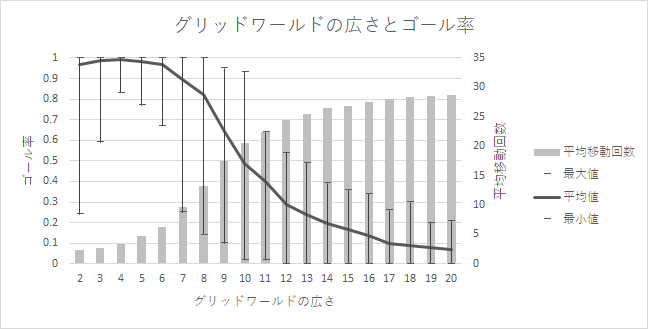
\includegraphics[scale=1.5]{img/valN.png}
  \end{center}
\end{figure}

グリッドワールドの大きさが2,3のときは一度通ったセルに戻ることを学習してしまい無限ループに入ることがあるためゴール率の低値が低くなったが,基本的にはグリッドワールドを大きくすればするほどゴール率の平均値が下がった.

\subsection{ゴールの位置の変更と学習後のゴール率}

\begin{figure}[ht]
  \begin{center}
    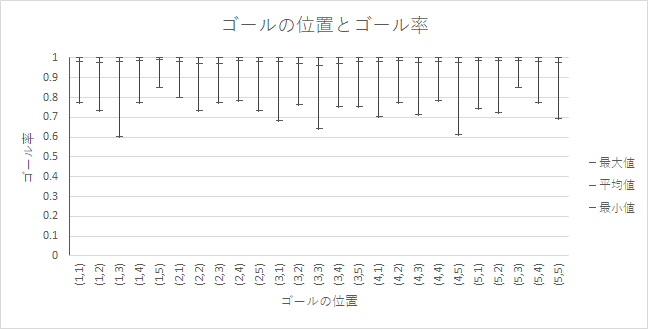
\includegraphics[scale=1.5]{img/valGoal.png}
  \end{center}
\end{figure}

結果はすべてゴール率が最大値は1で平均値は0.9後半の値となった.最低値はバラバラであり,位置によっての規則性はなさそうである.

\newpage

\subsection{履歴の長さの変更と学習後のゴール率}

\begin{figure}[ht]
  \begin{center}
    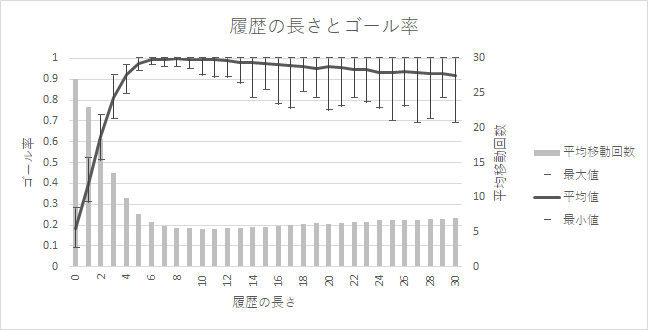
\includegraphics[scale=1.5]{img/valT.png}
  \end{center}
\end{figure}

履歴の長さの変更によるゴール率の平均値は7までは増加傾向にあり,10以降から減少する傾向があった.

\subsection{エージェントの寿命の変更と学習後のゴール率}

\begin{figure}[ht]
  \begin{center}
    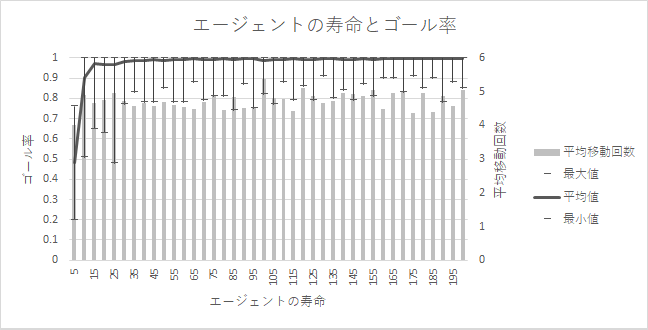
\includegraphics[scale=1.5]{img/valAgentLifetime.png}
  \end{center}
\end{figure}

エージェントの寿命の変更によるゴール率の平均値の変化は65までは増加する傾向があり,その後値はほぼ変化しない結果となった.

\newpage

\subsection{学習回数の変更と学習後のゴール率}

\begin{figure}[ht]
  \begin{center}
    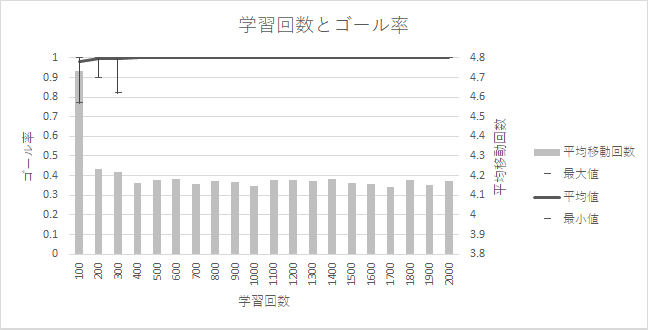
\includegraphics[scale=1.5]{img/valLearningLimit.png}
  \end{center}
\end{figure}

学習回数の変更によるゴール率の平均値の変化は400まで増加する傾向があり,その後は値は変化しない結果となった.

\subsection{報酬の変更と学習後のゴール率}

\begin{figure}[ht]
  \begin{center}
    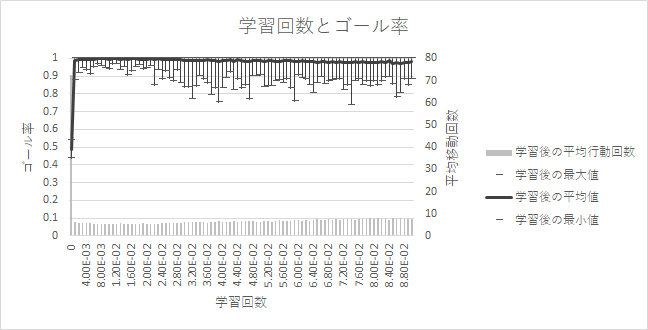
\includegraphics[scale=1.5]{img/valP.png}
  \end{center}
\end{figure}

報酬の変更によるゴール率の平均値は2.5e-2くらいまでは1に限りなく近づいていたがその後は離れていく結果となった.

\newpage

\subsection{更新ルールの変更と学習後のゴール率}

\begin{figure}[ht]
  \begin{center}
    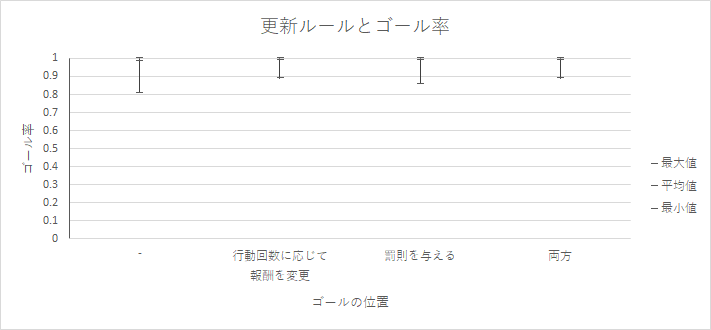
\includegraphics[scale=1.5]{img/valRule.png}
  \end{center}
\end{figure}

どれもゴール率の平均値はほぼ同じ数値となったが,行動数に応じて報酬を変更し罰則を与えたときが最も良い結果となった.

\subsection{まとめ}

以上の考察と評価の結果をもとにグリッドサイズが5のときに学習に最適なパラメータを考えた.以下の数値がそのパラメータである.

\begin{verbatim}
$ cat ./main.rb | head -n 16 | tail -n 14
# 定数
N = 5  # グリッドサイズ
GOAL_X = 3  # ゴールのX座標
GOAL_Y = 3  # ゴールのY座標
LEARNING_LIMIT = 500  # 学習回数
AGENT_LIFETIME = 1000  # エージェントの寿命
P = 3e-2  # 報酬
T = 4  # 報酬で矢印を遡ることができる回数
VAL = 100   # 評価を行う回数
# オプション
USE_SEED = true  # 固定された疑似乱数を使用する
RAND_GOAL = false  # ゴール位置をランダムにする
SHOW_DETAIL = false  # 実験の結果など詳細を表示させる
TRIAL_LIMIT = 100  # 実験回数,ARROWSがTRUEのとき無効
\end{verbatim}

それぞれの実験の結果を表示するときとしないときの結果は以下のようになった.

\newpage

\begin{verbatim}
SHOW_DETAIL: true
グリッドサイズ: 5, 学習回数: 500, エージェントの寿命: 1000,
報酬: 0.03, 履歴: 4, 評価回数: 100,
シード値: 固定, ゴール: 固定

[[0, 6, 0, 3], [0, 6, 0, 2], [0, 10, 0, 0], [0, 2, 5, 1], [0, 5, 4, 0]],
[[0, 10, 0, 0], [0, 10, 0, 0], [0, 10, 0, 0], [0, 0, 10, 0], [0, 3, 5, 0]],
[[0, 0, 0, 10], [0, 0, 0, 10], [2, 2, 2, 2], [0, 0, 10, 0], [0, 0, 10, 0]],
[[8, 0, 0, 1], [1, 0, 0, 7], [10, 0, 0, 0], [0, 0, 10, 0], [2, 1, 5, 0]],
[[6, 0, 0, 3], [5, 0, 1, 3], [10, 0, 0, 0], [9, 0, 0, 0], [2, 0, 7, 0]],

下下下左下
下下下左左
右右ゴ左左
上右上左左
上上上上左

学習時のゴール率: 1.0
学習時のエージェントの平均行動回数: 4.25
学習後のゴール率: 1.0
学習後のエージェントの平均行動回数: 2.37
\end{verbatim}

\begin{verbatim}

SHOW_DETAIL: false
学習時のゴール率の最大値: 1.0
学習時のゴール率の平均値: 1.0
学習時のゴール率の最小値: 1.0
学習時の平均移動回数: 4.148960000000002
学習後のゴール率の最大値: 1.0
学習後のゴール率の平均値: 1.0
学習後のゴール率の最小値: 1.0
学習後の平均移動回数: 2.4977999999999994
\end{verbatim}

\newpage

\section{グリッドサイズが10のときの学習に最適なパラメータ}

次にグリッドワールドの大きさが10のときの学習に最適なパラメータを調べた.これまでと同様に学習時と学習後のパラメータの変更によるゴール率の変化を以下のパラメータをもとに調べた.

\begin{verbatim}
# 定数
N = 10  # グリッドサイズ
GOAL_X = 5  # ゴールのX座標
GOAL_Y = 5  # ゴールのY座標
LEARNING_LIMIT = 500  # 学習回数
AGENT_LIFETIME = 100  # エージェントの寿命
P = 1e-2  # 報酬
T = 15  # 報酬で矢印を遡ることができる回数
VAL = 500   # 評価を行う回数
# オプション
USE_SEED = true  # 固定された疑似乱数を使用する
RAND_GOAL = false  # ゴール位置をランダムにする
SHOW_DETAIL = false  # 実験の結果など詳細を表示させる
TRIAL_LIMIT = 100  # 実験回数,ARROWSがTRUEのとき無効
\end{verbatim}

\newpage

\subsection{履歴の長さとゴール率}

履歴の長さを0から50まで1ずつ増やして学習を行ったときの学習中と学習後のゴール率はそれぞれ以下のようになった.

\begin{figure}[ht]
  \begin{center}
    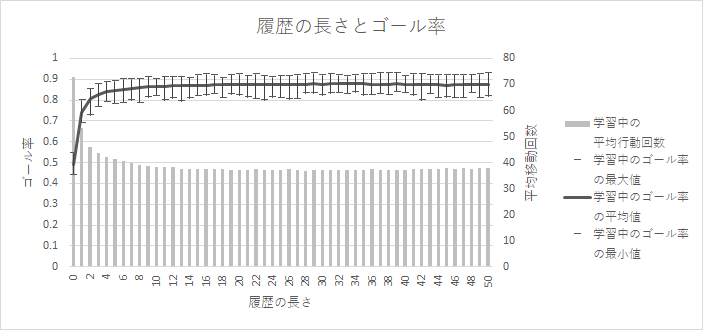
\includegraphics[scale=1.5]{img/changeT10.png}
  \end{center}
\end{figure}

\begin{figure}[ht]
  \begin{center}
    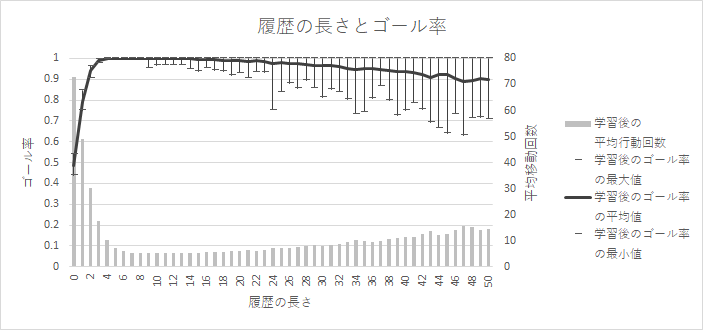
\includegraphics[scale=1.5]{img/valT10.png}
  \end{center}
\end{figure}

今回の学習後の結果と以前の結果を見ても,履歴の長さは角がギリギリ学習できるくらいの大きさに設定するのが一番効率の良い学習と考えられる.

\newpage

\subsection{エージェントの寿命とゴール率}

エージェントの寿命を5から200まで5ずつ増やして学習を行ったときの学習中と学習後のゴール率はそれぞれ以下のようになった.

\begin{figure}[ht]
  \begin{center}
    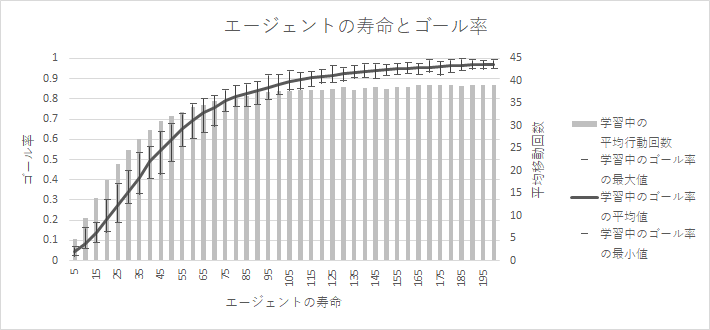
\includegraphics[scale=1.5]{img/changeAgentLifetime10.png}
  \end{center}
\end{figure}

\begin{figure}[ht]
  \begin{center}
    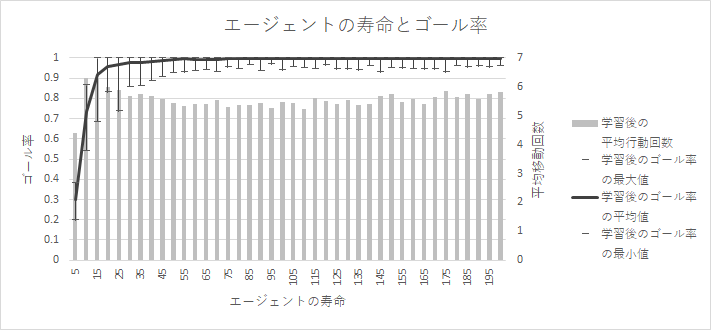
\includegraphics[scale=1.5]{img/valAgentLifetime10.png}
  \end{center}
\end{figure}

今回の学習後の結果と以前の結果を比較すると,同じ形のグラフになっていることがわかる.しかし,前回と今回の結果から学習後のゴール率の平均値が変化しなくなる値を特定する法則はわからなかった.そのため,学習の最適なエージェントの寿命はこのようにグラフを作成して見つけるか,処理時間を気にしないのであれば大きい値を取る方法が良い方法と考えられる.

\newpage

\subsection{学習回数とゴール率}

学習回数を100から2000まで100ずつ増やして学習を行ったときの学習中と学習後のゴール率はそれぞれ以下のようになった.

\begin{figure}[ht]
  \begin{center}
    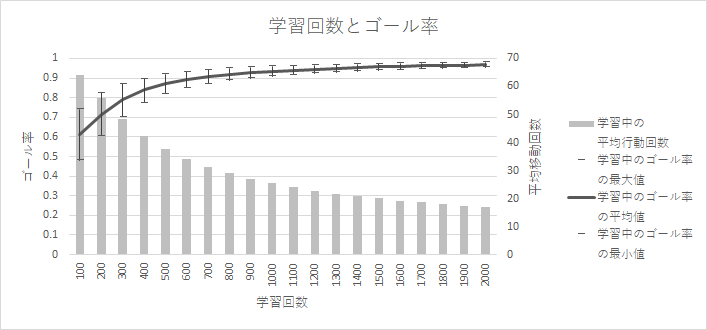
\includegraphics[scale=1.5]{img/changeLearningLimit10.png}
  \end{center}
\end{figure}

\begin{figure}[ht]
  \begin{center}
    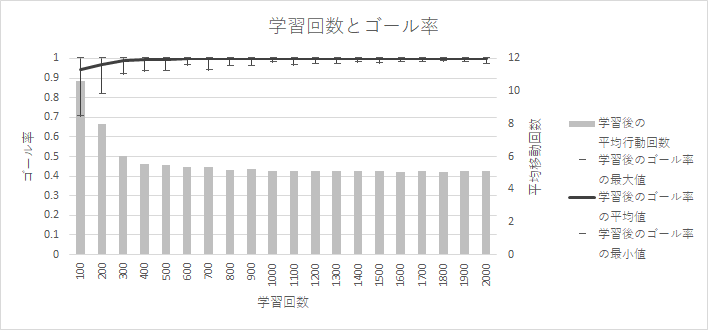
\includegraphics[scale=1.5]{img/valLearningLimit10.png}
  \end{center}
\end{figure}

今回の学習後の結果と以前の結果を比較すると,同じような形のグラフになっていることがわかる.しかし,学習後のゴール率の平均値があまり変化しなくなる値を特定する法則はわからなかった.そのため,学習の最適な学習回数はこのようにグラフを作成して見つけるか,処理時間を気にしないのであればとりあえず大きい値を取る方法が良い方法と考えられる.

\newpage

\subsection{報酬とゴール率}

報酬を$0$から$9e-2$まで$1e-3$ずつ増やして学習を行ったときの学習中と学習後のゴール率はそれぞれ以下のようになった.

\begin{figure}[ht]
  \begin{center}
    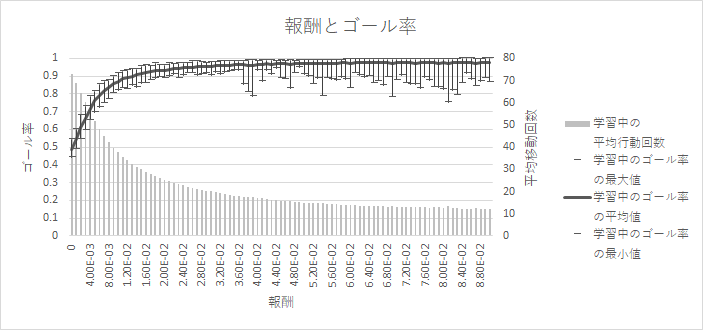
\includegraphics[scale=1.5]{img/changeP10.png}
  \end{center}
\end{figure}

\begin{figure}[ht]
  \begin{center}
    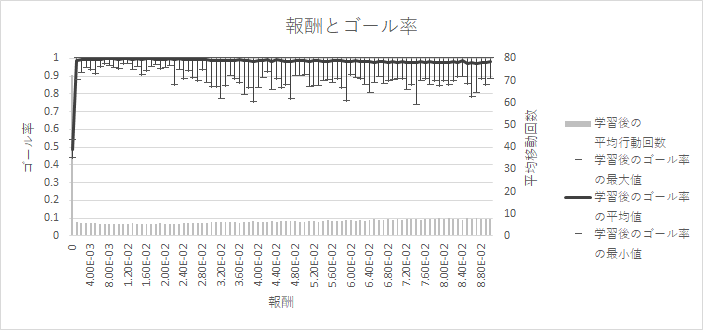
\includegraphics[scale=1.5]{img/valP10.png}
  \end{center}
\end{figure}

今回の学習後の結果と以前の結果を比較すると,同じような形のグラフになっていることがわかる.しかし,学習後のゴール率の平均値があまり変化しなくなる値を特定する法則はわからなかった.そのため,学習の最適な学習回数はこのようにグラフを作成して見つける方法が良い方法と考えられる.

\newpage

\subsection{まとめ}

上記の結果から,グリッドサイズが10のときの学習に最適なパラメータは以下のようになった.

\begin{verbatim}
$ cat ./main.rb | head -n 16 | tail -n 14
# 定数
N = 10  # グリッドサイズ
GOAL_X = 5  # ゴールのX座標
GOAL_Y = 5  # ゴールのY座標
LEARNING_LIMIT = 700  # 学習回数
AGENT_LIFETIME = 85  # エージェントの寿命
P = 1e-2  # 報酬
T = 10  # 報酬で矢印を遡ることができる回数
VAL = 500   # 評価を行う回数
# オプション
USE_SEED = true  # 固定された疑似乱数を使用する
RAND_GOAL = false  # ゴール位置をランダムにする
SHOW_DETAIL = false  # 実験の結果など詳細を表示させる
TRIAL_LIMIT = 100  # 実験回数,ARROWSがTRUEのとき無効
\end{verbatim}

このパラメータで行動回数に応じて履歴を遡る回数を変更する更新ルールを使用して学習をさせると結果は以下のようになった.

\begin{verbatim}
SHOW_DETAIL: true
グリッドサイズ: 10, 学習回数: 700, エージェントの寿命: 85,
報酬: 0.01, 履歴: 10, 評価回数: 500,
シード値: 固定, ゴール: 固定

[[0, 4, 0, 5], [0, 3, 3, 3], [0, 3, 3, 3], [0, 3, 3, 3], [0, 3, 3, 2], [0, 3, 3, 2], [0, 3, 3, 3], [0, 3, 3, 3], [0, 3, 3, 3], [0, 4, 5, 0]],
[[3, 3, 0, 3], [2, 2, 2, 2], [2, 2, 2, 2], [1, 3, 1, 3], [1, 5, 1, 1], [1, 3, 2, 2], [2, 3, 2, 1], [2, 2, 2, 2], [2, 2, 2, 2], [3, 3, 3, 0]],
[[2, 3, 0, 3], [1, 3, 2, 2], [1, 3, 1, 3], [1, 3, 1, 2], [0, 7, 0, 1], [1, 4, 2, 1], [1, 3, 2, 1], [2, 2, 3, 1], [2, 2, 2, 2], [3, 3, 3, 0]],
[[3, 3, 0, 3], [1, 2, 1, 3], [1, 1, 1, 5], [0, 5, 0, 2], [0, 10, 0, 0], [0, 1, 7, 0], [0, 1, 7, 0], [1, 2, 4, 1], [2, 2, 3, 2], [2, 3, 3, 0]],
[[2, 2, 0, 4], [1, 1, 1, 4], [0, 0, 0, 8], [0, 0, 0, 10], [2, 2, 2, 2], [0, 0, 10, 0], [1, 0, 7, 0], [1, 1, 6, 1], [2, 1, 4, 1], [2, 2, 4, 0]],
[[3, 2, 0, 3], [2, 1, 1, 3], [3, 1, 1, 3], [2, 1, 1, 5], [10, 0, 0, 0], [4, 0, 3, 0], [2, 1, 3, 1], [2, 1, 3, 1], [2, 2, 3, 2], [3, 2, 3, 0]],
[[3, 3, 0, 3], [3, 2, 1, 2], [2, 1, 2, 3], [4, 1, 1, 2], [8, 0, 0, 0], [4, 1, 2, 1], [3, 1, 3, 1], [2, 2, 2, 2], [2, 2, 2, 2], [3, 3, 3, 0]],
[[3, 3, 0, 3], [2, 2, 2, 2], [3, 1, 2, 2], [3, 1, 1, 2], [5, 1, 1, 1], [3, 1, 3, 1], [3, 2, 3, 1], [2, 2, 2, 2], [2, 2, 2, 2], [3, 3, 3, 0]],
[[3, 3, 0, 3], [2, 2, 2, 2], [2, 2, 2, 2], [3, 2, 2, 2], [3, 1, 2, 2], [3, 2, 2, 2], [2, 2, 2, 2], [2, 2, 2, 2], [2, 2, 2, 2], [3, 3, 3, 0]],
[[5, 0, 0, 4], [3, 0, 3, 3], [3, 0, 3, 3], [3, 0, 3, 3], [3, 0, 3, 3], [3, 0, 3, 3], [3, 0, 3, 3], [3, 0, 3, 3], [3, 0, 3, 3], [4, 0, 5, 0]],

右下下下下下下下左左
下下右右下下下下左左
下下右下下下下左左下
下右右下下左左左左下
右右右右ゴ左左左左左
右右右右上上左左左上
右上右上上上上左左上
上右上上上上左左上左
上右右上上上上上左上
上右上上上上上左上左

学習時のゴール率: 0.8585714285714285
学習時のエージェントの平均行動回数: 32.644285714285715
学習後のゴール率: 1.0
学習後のエージェントの平均行動回数: 5.128
\end{verbatim}

\begin{verbatim}

SHOW_DETAIL: false
学習時のゴール率の最大値: 0.9128571428571428
学習時のゴール率の平均値: 0.8689714285714285
学習時のゴール率の最小値: 0.8185714285714286
学習時のゴール率の平均行動回数: 31.698571428571416
学習後のゴール率の最大値: 1.0
学習後のゴール率の平均値: 1.0
学習後のゴール率の最小値: 1.0
学習後のゴール率の平均行動回数: 5.051519999999999
\end{verbatim}

エージェントの寿命を短くしたため学習時のゴール率は1にならなかったが,学習後のゴール率は1にすることができた.

\end{document}
